\documentclass[a4paper,11pt]{article}
\usepackage[utf8]{inputenc}
\usepackage[T1]{fontenc}
\usepackage[french]{babel}
\usepackage[right=2.5cm, left=2.5cm, bottom=4cm, top=3cm]{geometry}
\usepackage{textcomp}
\usepackage{graphicx}
\usepackage{mathtools,amssymb,amsthm}
\usepackage{lmodern}
\usepackage{multirow}
\usepackage{array}
\usepackage{longtable}

\title{\vspace{13em}{\huge Rapport Final}}
\author{Edouard Fouassier - Maxime Gonthier - Benjamin Guillot\\
		Laureline Martin - Rémi Navarro - Lydia Rodrigez de la Nava
		\vspace{2em}\\
		Algorithme Génétique
		\vspace{2em}}

\begin{document}
	
	\pagenumbering{gobble}\clearpage
	\maketitle\vspace{13em}
\newpage
\tableofcontents
\newpage\clearpage\pagenumbering{arabic}

	\section{Introduction}
		Dans le cadre du module IN608 du dernier semestre de notre Licence Informatique à l’UVSQ, nous avons eu l’occasion de réaliser un projet sous la direction de Mme Leila Kloul.\\
		Nous avons choisi, parmi les sujets proposés, le sujet Algorithme Génétique car c’est un sujet qui demande à la fois des connaissances basiques en biologie et des connaissances plus poussées en algorithmique, ce qui nous a beaucoup plu.
		De plus c’est un sujet qui demande de transformer en programmation des méthodes biologiques, ce qui est un défi intéressant.\\
		
		Notre projet consiste à créer un logiciel permettant à un utilisateur de résoudre un problème d’optimisation grâce à un Algorithme Génétique.\\
		Mais tout d’abord, qu’est-ce qu’un Algorithme Génétique ?\\
		C’est en 1960 que John Holland, professeur à l’Université du Michigan, commence à étudier la création d’un algorithme qui s’inspire de la théorie de l’évolution de Darwin, et qui résoudrait des problèmes d’optimisation de manière efficace.
		Le premier livre faisant part du sujet, Adaptation in Natural and Artificial System, fut publié en 1975 mais l’algorithme ne sera rendu populaire qu’en 1989, lors de la publication de Genetic Algorithms in Search, Optimization, and Machine Learning par David Goldberg.
		Un algorithme génétique, ou AG, s’inspire de la nature en se basant sur la sélection naturelle, c’est-à-dire qu’une population est composée d’individus qui ont plus ou moins de chance d’être sélectionnés pour se reproduire dans le but de créer de nouveaux individus de la prochaine génération.
		De cette façon, au bout d’un certain nombre d’itérations de cette sélection, les individus les plus forts seront les résultats les plus adaptés au problème.\\
		Les AG sont entre autres utilisés dans le domaine de la génétique, pour résoudre une fonction mathématique, pour optimiser un portefeuille ou encore dans le domaine de l’apprentissage.\\
		L’objectif de notre projet est donc d’implémenter un tel algorithme pour permettre à un utilisateur d’entrer des données à son problème et d’obtenir les résultats de ce dernier en sortie.
		Pour cela, il fallait tout d’abord une interface dans laquelle l’utilisateur entre une par une ses données, ou entre un fichier où sont déjà enregistrées ses données.
		Il fallait aussi que l’algorithme soit générique pour pouvoir prendre en charge un maximum de problèmes.\\
		Le logiciel se veut ergonomique avec une interface intuitive, qui ne nécessite pas de prérequis autre qu’une ou deux fonctions à optimiser.
		Pour le reste des données, l’utilisateur sera guidé dans le manuel d’utilisation pour utiliser les données les plus efficaces au fonctionnement de l’AG.\\
		Une itération de l’algorithme génétique comporte plusieurs étapes : l’évaluation des individus : à chaque individu est attribué un score par rapport à la ou les fonctions d’évaluation donnée(s) par l’utilisateur, ensuite la sélection des individus qui pourront créer de nouveaux individus, puis le croisement de deux individus sélectionnés, ou crossover, qui auront un probabilité plus ou moins élevée d’être mutés.\\
		Nous avons choisi d’implémenter notre logiciel dans le langage de programmation C++ car c’est un langage hybride. Il était nécessaire d’avoir une partie procédurale pour effectuer les calculs sur les individus, pour les tests et pour la gestion des fichiers d’entrées / de sortie. Il fallait aussi une partie objet pour l’implémentation des individus et de la population.
	
	\section{Explication de l’architecture}
		\underline{Organigramme :}\\
		\centerline{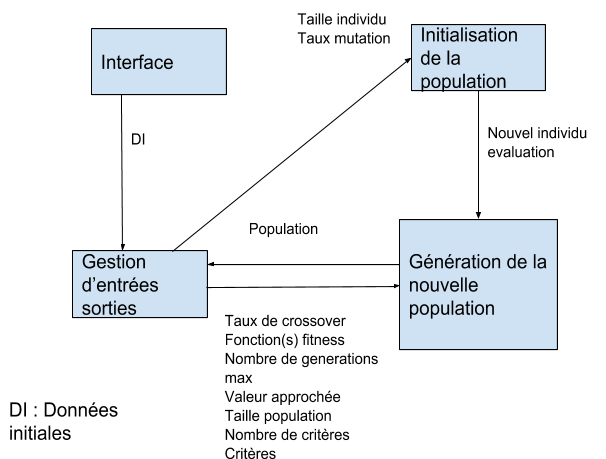
\includegraphics[scale = 0.5]{OrganigrammeV9.png}}\\
		
		Notre logiciel est organisé en 4 modules :\\
		\begin{itemize}
			\item L’initialisation de la population
			\item La génération d’une nouvelle population
			\item La gestion des fichiers d’entrées et sorties
			\item L’interface\\
		\end{itemize}
		Le module Interface est implémenté avec le logiciel Qt et est par conséquent une classe.\\
		Les modules d’initialisation de la population et de génération de nouvelle population sont toutes deux des classes qui implémentent respectivement les individus et une population.\\
		Le choix d’en faire des classes a été motivé par les possibilité de manipulation offertes de ces des notions en temps qu’objet.
		Un Individu et une Population étant composé de plusieurs éléments, l’utilisation de classe nous a permis d’en faire des attributs de ces classes tel que l’ensemble de chromosome pour un Individu ou l’ensemble d’individu pour une population.\\\\
		
		Le module de gestion d’entrées sorties est quant à lui le seul module procédural du projet. Ce module contient de la lecture, de l’écriture et des calculs ce qui est plus simple à implémenter en procédural. \\
		
		\subsection{Initialisation de la population}
			Un individu est dans notre logiciel implémenté comme un tableau de gènes qui peuvent prendre comme valeur 0 ou 1.
			Ce tableau est de la taille entrée par l’utilisateur avec une case ajoutée au début du tableau pour le signe (0 est positif, 1 est négatif).
			Chaque individu a aussi son score et son rang, en fonction du critère.\\
			La classe Individu a aussi trois éléments statiques : probabilité de mutation, taille de l’individu et nombre de critères.
			Ceux-ci sont récupérés grâce au module de gestion d’entrée et sortie qui envoie un tableau de trois cases contenant ces éléments.\\
			L’individu peut être initialisé à 0 ou bien peut être créé de manière aléatoire. Cette dernière option est notamment utilisée pour créer la toute première population de l’AG.\\
			C’est dans ce module qu’un individu est évalué.
			En effet, il est d’abord décodé puis entré dans la fonction fitness pour obtenir le score.
			Une fois l’individu créé ou évalué, il est envoyé au module de Génération d’une population.
		
		\subsection{Génération de la nouvelle population}
		
			Le rôle de ce module est de générer une population.
			Une population est un vecteur d’individus, initialisé en fonction des données envoyées par le module de gestion d’entrée et sortie (cf l’organigramme).\\
			Ce module effectue de plus les tests qui permettent de savoir s’il faut continuer ou pas l’itération de l’AG.
			Il teste notamment si le nombre de génération à créer a été atteint ou si les résultats convergent, auxquels cas l’AG s’arrête et le module de gestion d’entrée et sortie écrit le fichier de résultats final.\\
			De plus, c’est dans ce module qu’on retrouve les opérateurs principaux de l’algorithme génétique.
			En effet, on y trouve la sélection pour laquelle on évalue les individus puis on les trie par rapport à leur score afin d’effectuer une sélection par rang.
			On y trouve aussi le crossover qui se sert de sélection pour choisir deux individus et les croiser, puis ajouter les nouveaux individus dans la population.
			Le choix de la technique utilisée pour chacun de ces outils seront expliqués plus tard dans le rapport.\\
			Avec tous ces opérateurs, on peut donc générer une nouvelle population.\\
			Une fois que celle-ci est pleine, elle est évaluée puis envoyée au module de gestion d’entrée et de sortie pour écrire les scores de chaque individu et les statistiques de la population.\\

			Afin de réaliser notre application, nous avons été confrontés à plusieurs contraintes et choix. Nous avons dû par exemple choisir entre plusieurs algorithmes de sélection ou plusieurs algorithmes de crossover.\\
			Pour la sélection des individus, plusieurs choix s’offraient à nous. Parmis eux se trouvaient la sélection par roulette, la sélection élitiste, la sélection par tournoi et la sélection uniforme.
			La sélection élitiste choisit uniquement les meilleurs individus, donc le hasard n’est pas du tout pris en compte, ce qui ne correspondait pas à notre objectif d’inclure une part de hasard comme la sélection naturelle.
			La sélection par tournoi confronte les individus deux à deux et choisit le meilleur score.
			Cette sélection inclut une part de hasard mais les scores les plus faibles seront toujours absents de la sélection.
			La sélection uniforme est complètement aléatoire et ne permet donc pas d’optimiser nos résultats.
			Ainsi nous avons choisis la sélection par rang, qui est une forme de sélection par roulette qui inclut une part de hasard tout en sélectionnant majoritairement les meilleurs individus.\\
			Pour le crossover nous avions le choix entre un croisement en un point ou multipoint.
			Nous avons choisis le crossover à un seul point car il permet d’éviter une convergence prématurée. De plus cette technique est plus proche de la réalité biologique.

		\subsection{Gestion d'entrée sortie}
			Le module gestion d’entrée et sortie se charge de tout ce qui touche à l’écriture ou la lecture dans un fichier.\\
			On a vu précédemment que le module de gestion d’entrée et sortie recevait du module interface soit les données une à une soit un fichier de données.
			Dans le premier cas, le module se charge de les écrire dans un nouveau fichier.
			Dans le deuxième cas, on parcourt le fichier pour vérifier que toutes les données sont cohérentes. Dans les deux cas, le module vérifie que la fonction fitness est parsable.
			Pour qu’une fonction soit parsable elle doit être correctement parenthésée, ne pas avoir de division par zéro, avoir correctement orthographié les fonctions mathématiques et n’avoir qu’une seule variable nommée obligatoirement ‘x’.\\
			Une fois toutes ces données vérifiées, le module se charge d’envoyer toutes les données nécessaires au fonctionnement du module d’initialisation de la population et au module de génération d’une population. /! A DEVELOPPER\\
			A chaque itération de l’algorithme génétique, le module reçoit de Génération d’une population la population qui vient d’être créée.
			Il prend celle-ci et écrit le score de chaque individu dans un fichier.\\
			Le module calcule ensuite les statistiques d’une population, c’est-à-dire qu’il écrit le score du meilleur individu, du moins bon et fait un moyenne pondérée de toute la population.\\
			En s’aidant des statistiques précédemment obtenues, à la fin du programme, le module va écrire dans le(s) format(s) souhaité(s) par l’utilisateur le fichier final qui fait une synthèse du déroulement de l’algorithme et aussi le résultat à son problème.
		
		\subsection{Interface}
			Le module interface est le module qui s’occupe de la création et de l’affichage des champs de saisie. Nous avons utilisé Qt pour la créer car /! À JUSTIFIER\\	
			L’interface laisse le choix à l’utilisateur d’entrer ses données une par une, ou bien d’entrer le chemin  d’un fichier où celles-ci se trouvent.
			Le module vérifie que les données écrites sont correctes directement dans l’interface dans le premier cas.
			On étudiera en détail dans la partie Description du fonctionnement quelles données sont nécessaires.\\

			Le module présente également à l’utilisateur plusieurs boutons.
			Tout d’abord le bouton Aide qui ouvrira le manuel d’utilisation au cas où l’utilisateur a un doute sur l’utilisation de l’interface.\\
			Le bouton Lancer lance l’algorithme génétique si toutes les données sont correctes.
			Autrement l’utilisateur est prévenu de ses erreurs et retourne sur l’interface pour les corriger.\\
			Le bouton Arrêter arrête l’itération de l’AG lancé, mais enregistre les données et fournit le fichier de sortie malgré tout.\\
			Le bouton Quitter quant à lui arrête l’AG sans rien enregistrer.\\
			Dans le cas où l’utilisateur a entré ses données dans les champs de saisie de l’interface, celles-ci sont envoyées au module d’entrée et sortie pour qu’elles soient enregistrées dans un fichier.
			Dans le cas où l’utilisateur a entré directement un fichier de données, le nom de ce dernier est envoyé au module d’entrée et sortie qui se chargera de vérifier la cohérence des données.\\

\end{document}
